\documentclass[a4paper,12pt]{report}

\usepackage[utf8]{inputenc}
\usepackage[russian]{babel}
\inputencoding{utf8}
\usepackage{graphicx}
\usepackage{caption}
\usepackage{subcaption}
\usepackage{float}
\graphicspath{{images/}}

\makeatletter
\renewcommand\chapter{\par%
\thispagestyle{plain}%
\global\@topnum\z@
\@afterindentfalse
\secdef\@chapter\@schapter}
\makeatother

\usepackage{geometry} % Меняем поля страницы
\geometry{left=2cm}% левое поле
\geometry{right=1.5cm}% правое поле
\geometry{top=3cm}% верхнее поле
\geometry{bottom=2cm}% нижнее поле

\begin{document}

\begin{titlepage}
\begin{center}
\vspace{8cm}
Санкт-Петербургский Государственный Университет. \\ Математико-Механический факультет. \\ Кафедра астрономии. \\
\vspace{2cm}
Мазурин К.Э. \\
\vspace{1cm}
\Large
{\bf ‘’Исследование алгоритмов преобразования координат на примере программных пакетов SOFA и NOVAS.’’\\ Курсовая работа, 4-й курс. } \\
\vspace{1cm}
Научный руководитель -- Петров Сергей Дмитриевич.\\
\vspace{13cm}
Санкт-Петербург -- 2016 год.
\end{center}
\end{titlepage}

{\large\tableofcontents}
\newpage

\large
\chapter*{Введение}
\addcontentsline{toc}{chapter}{Введение}
Задача координатного преобразования между земной и небесной системами координат широко применима в астромерии. Без этого не обойтись при вычислении
положений космических аппаратов, к примеру, спутников GPS и ГЛОНАСС; при уточнении параметров ориентации Земли (ПОЗ) с помощью РСДБ наблюдений и в многих
других случаях. Наиболее часто при работе с космическими аппаратами используют системы GCRS (Geocentric Celestial Reference System - геоцентрическая
небесная система координат) и ITRS (International Terrestrial Reference System - международная земная система координат).

\section*{Немного о системах отсчета}
{\bf BCRS} - небесная система координат, окончательно принятая Международным Астрономическим Союзом в качесте основной небесной СК в конце 
1990-х годов. Имеет фиксированные оси с началом отсчета в барицентре Солнечной системы. Главная плоскость максимально приближена к небесному экватору на эпоху J2000.0,
а начало отсчета прямых восхождений приближено, насколько это возможно, к точке весеннего равноденствия на эпоху J2000.0. \newline {\bf GCRS} - модификация этой системы координат.
Ее отличие от {\it BCRS} в том, что начало отсчета расположено не в барицентре Солнечной Системы, а в геоцентре Земли, что позволяет легче работать с околоземными телами. \newline
{\bf ITRS} - международная земная система координат, принятая МАС в 1991 году. Начало отсчета расположено в геоцентре Земли, основная плоскость - земной экватор (ось Z направлена 
в опорный полюс Земли, ось X лежит в плоскости опорного меридиана, расположенного в 5".3 к востоку от Гринвичского меридиана). Система вращается вместе с Землей и не является инерциальной.
\newpage
\chapter*{Кратко об алгоритмах координатного преобразования}
\addcontentsline{toc}{chapter}{Кратко об алгоритмах координатного преобразования}
Существует два вида алгоритмов преобразования координат из системы ITRS в GCRS (и наоборот). Их различие состоит в том, что за начало отсчета прямых восхождений принимают либо
точку весеннего равноденствия (традиционный метод), либо т.н. CIO (Celestial Intermediate Origin - практически неподвижную точку на экваторе CIP - среднего полюса). Подробнее
о новой концепции можно прочитать в \cite{iers} и \cite{capit}.
\newline В общем виде оба алгоритма представляют собой композицию нескольких вращений:
\begin{equation}
[GCRS] = Q(t)R(t)W(t) * [ITRS],
\end{equation}
где $[GCRS]/[ITRS]$ - вектор положения в системе GCRS/ITRS, $Q(t)$ - матрица преобразования, связанного с движением небесного полюса в небесной системе координат,
$R(t)$ - матрица преобразования, связанного в суточным вращением Земли, и $W(t)$ - матрица преобразования, связанного с движением полюса в теле Земли. Матрица обратного преобразования
получается простым обращением матрицы $Q(t)R(t)W(t)$.
\bigskip
Матрица $W(t)$ для обоих алгоритмов выглядит одинаково:
\begin{equation}
W(t) = R_3(-s')\dot R_2(x_p)\dot R_1(y_p),
\end{equation}
где $R_1, R_2, R_3$ - матрицы вращения вокруг осей 1, 2 и 3 соответственно, $(x_p, y_p)$ - координаты полюса (CIP) в теле Земли, а $s'$ - т.н. TIO locator - положение
TIO (Terrestrial Intermediate Origin - начало отсчета долгот в системе ITRS) на экваторе CIP.
\bigskip
Матрица $R(t)$ в CIO-based алгоритме выражается как:
\begin{equation}
R(t) = R_3(-ERA),
\end{equation}
где ERA (Earth Rotation Angle) - угол между CIO и TIO на экваторе CIP. Для традиционного алгоритма данная матрица выглядит схожим образом, только вместо ERA в ней используется
Apparent Greenwich Siderial Time - угол между точкой весеннего равноденствия и TIO, связанный с суточным вращением Земли.
\bigskip
Матрица $Q(t)$ для CIO-based алгоритма выглядит следующим образом:
\begin{equation}
Q(t) = R_3(-E)\dot R_2(-d)\dot R_3(E)\dot R_3(s),
\end{equation}
где E и d - это такие углы, что координаты CIP в системе GCRS выглядят слежующим образом:
\begin{equation}
X = sin(d)cos(E) \quad Y = sin(d)sin(E) \quad Z = cos(d),
\end{equation}
а s - т.н. CIO locator - положение CIO на экваторе CIP. Матрица $Q(t)$ для классического метода выражается через стандартную модель прецессии-нутации, подробнее об этом можно найти в \cite{iers}.

\chapter*{Реализация алгоритмов в SOFA и NOVAS}
\addcontentsline{toc}{chapter}{Реализация алгоритмов в SOFA и NOVAS}
\section*{NOVAS}
В программном пакете NOVAS данный алгоритм представлен двумя процедурами: ter2cel для перевода вектора положений из земной системы координат в небесную и cel2ter для обратного
преобразования. \newline
Рассмотрим процедуру cel2ter. На вход ей подаются следующие аргументы: jd\_ut\_high, jd\_ut\_low - юлианская дата в системе UT1, разделенная на две части произвольным образом, так 
что jd\_ut\_high + jd\_ut\_low = JD (подробнее об этом можно найти в \cite{sofa}); delta\_t - разность TT - UT1 на нужную дату; method = \{0,1\} - параметр, отвечающий за
то, какой метод будет использован (0 - CIO-based; 1 - классический); accuracy = \{0,1\} - параметр, отвечающий за точность метода (0 - полная точность; 1 - пониженная точность);
option = \{0,1\} - параметр, указывающий, к какой системе относится входной вектор: GCRS или к системе, связанной с экватором и точкой весеннего равноденствия (опция актуальна только 
для классического метода); $x_p, y_p$ - координаты полюса в угловых секундах; вектор в небесной системе координат и вектор в земной системе координат (который и будет результатом работы
процедуры). \newline
В CIO-based методе сначала вектор переводится в т.н. систему CIRS (Celestial Intermediate Reference System) путем домножения исходного вектора на базисные векторы этой системы. 
Последние получаются в результате работы процедуры cio\_basis. Затем при помощи процедуры era считается Earth Rotation Angle и к вектору в системе CIRS применяется поворот на этот угол 
(процедура spin). Получившийся вектор будет в т.н. системе TIRS (Terrestrial Intermediate Reference System). Финальным шагом преобразования является учет движения полюса в теле Земли. За это
отвечает процедура wobble. \newline
Классический метод реализован по тому же принципу. На первом шаге вектор переводится в систему CIRS путем последовательного применения к нему процедур frame\_tie, precession и nutation.
Далее ищется угол поворота Земли (GAST) при помощи процедуры siderial\_time, затем вызывается уже упомянутая процедура spin, результатом работы которой является вектор в системе TIRS.
Последний шаг точно такой же, как и в CIO-based методе - вызов процедуры wobble.

\section*{SOFA}


\chapter*{Проверка работы алгоритмов}
\addcontentsline{toc}{chapter}{Проверка работы алгоритмов}
Для того, чтобы убедиться в том, что оба пакета программ годятся для того, чтобы обрабатывать реальные астрометрические наблюдения, необходимо было выполнить проверку того, что 
оба алгоритма на одном и том же тестовом примере выдадут одинаковый результат. Рассматривается обратный алгоритм: перевод из небесной системы координат в земную. В качестве 
тестовых данных были взяты: вектор в небесной системе координат (0, 1000, 10000); координаты полюса (-0".002, 0".529); дата и время 17 часов 29.04.2016; для простоты разница TT - UT1 
была взята равной 0. Результаты работы двух программ показаны на рисунке:
\begin{figure}[H]
\centering
\begin{subfigure}{.5\textwidth}
\centering
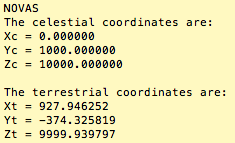
\includegraphics[width=.9\linewidth]{NOVAS.png}
\caption{NOVAS}
\label{fig:sub1}
\end{subfigure}%
\begin{subfigure}{.5\textwidth}
\centering
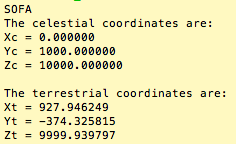
\includegraphics[width=.9\linewidth]{SOFA.png}
\caption{SOFA}
\label{fig:sub2}
\end{subfigure}
\caption{Результаты работы программ на тестовом примере.}
\label{fig:test}
\end{figure}

Как видно из рисунков, результаты работы программ совпадают с достаточно приличной точностью: отклонение составляет лишь единицы сантиметров. \newline
Также интересно было сравнить результаты работы алгоритма координатного преобразования для случаев традиционного и CIO-based методоов. Для проверки был взят пакет NOVAS и его обертка на языке
Python. В качестве тестового примера были взяты те же данные, что описаны выше. Кроме того, для сравнения также приведены результаты работы алгоритма для случая "пониженной точности",
который был введен для ускорения работы программы в ущерб точности вычислений (SOFA не предлагает данной опции). Результаты представлены на рисунке:
\begin{figure}[H]
\centering
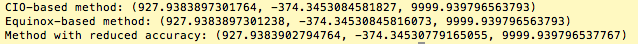
\includegraphics[width=.9\linewidth]{two_algs.png}
\caption{Результаты работы традиционного метода, CIO-based метода и метода с пониженной точностью}
\label{fig1}
\end{figure}

\chapter*{Заключение}
\addcontentsline{toc}{chapter}{Заключение}
Мною были исследованы алгоритмы координатного преобразования. Были рассмотрены и изучены программные пакеты, реализующие данные алгоритмы. Также было проведено сравнение
работы этих программных пакетов, по результатам которого можно сделать вывод, что они пригодны для использования в реальных астрометрических задачах.

\newpage
\addcontentsline{toc}{chapter}{Литература}
\begin{thebibliography}{9}

\bibitem{iers}
    International Earth Rotation and Reference Systems Service,
    \emph{IERS Conventions 2010}.
    Verlag des Bundesamts f\"{u}r Kartographie und Geod\"{a}sie, Frankfurt am Main,
    2010.

\bibitem{capit}
	N.Capitaine,
	\emph{Definition and realization of the celestial intermediate reference system}.
	International Astronomical Union,
	2008

\bibitem{novas}
    \emph{User's guide to NOVAS Version C3.1}.
    U.S. Naval Observatory,
    2011.

\bibitem{sofa}
	International Astronomical Union,
	\emph{The SOFA software libraries}.
	2015.

\end{thebibliography}

\end{document}
